\section{Material e métodos}

\begin{frame}{Material e métodos}{Liga estudada}
  \begin{columns}
    \begin{column}{.6\textwidth}
      \begin{itemize}
        \item Liga fundida como blocos em ``Y'' na Tupy Fundições S.A.
        % \item Microestrutura original ferrítico-perlítica
        \item 3,5\%C, 2,5\%Si, \textbf{0,2\%Mn}, 0,4\%Cu; impurezas (P + S + Cr < 0,1\%)
        \item Inoculação: > 400 nódulos/mm\textsuperscript{2}
      \end{itemize}
    \end{column}

    \begin{column}{.4\textwidth}
      \begin{figure}
        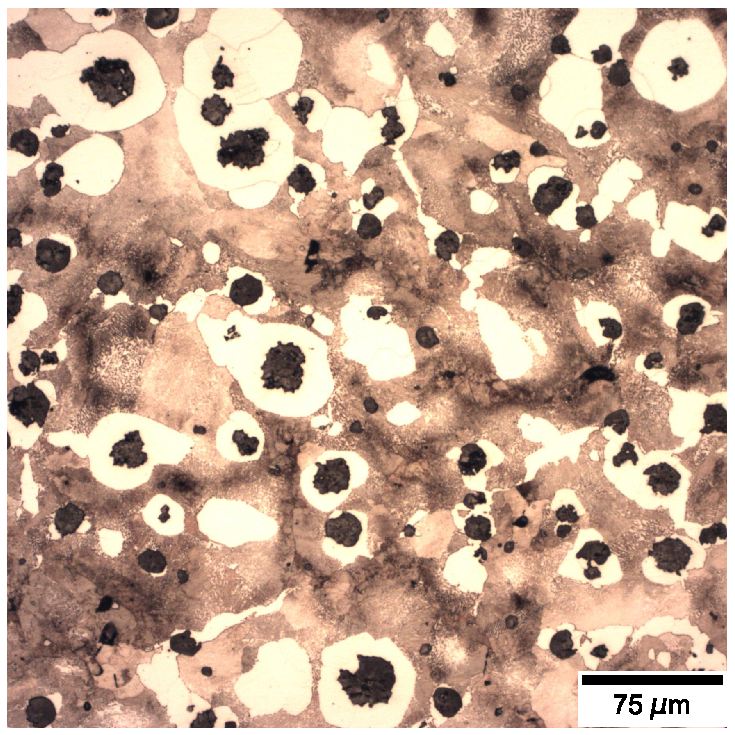
\includegraphics[width=\textwidth]{../tese/img/micrografias/CR/200x-1_scalebar.pdf}
      \end{figure}
    \end{column}
  \end{columns}
\end{frame}

\begin{frame}{Material e métodos}{Dilatometria}
  \begin{itemize}
    \item Dilatômetro Bähr 805A, aquecimento por indução \& resfriamento gás He $\rightarrow$ controle acurado de temperatura
    \item CP cilíndrico \O 4mm, L = 10mm
    \item Aquisição em tempo real da dilatação da amostra $\rightarrow$ cinética de transformação
  \end{itemize}
\end{frame}

\begin{frame}{Material e métodos}{Dilatometria}
  \begin{itemize}
    \item $T_A$ = \SI{880}{\degreeCelsius} no campo $\gamma + grafita$. Thermo-Calc\textregistered{} $\rightarrow$ 0,76\%C em $\gamma$
    \item \textbf{$T_T$ = 140, 170 e 200~\SI{}{\degreeCelsius}}
    \item \textbf{$T_P$ = 300, 375 e 450~\SI{}{\degreeCelsius}}
    \item \textbf{$t_P$ = 0, 30~s, 5~min, 15~min, 2~h}
  \end{itemize}

  \begin{figure}
    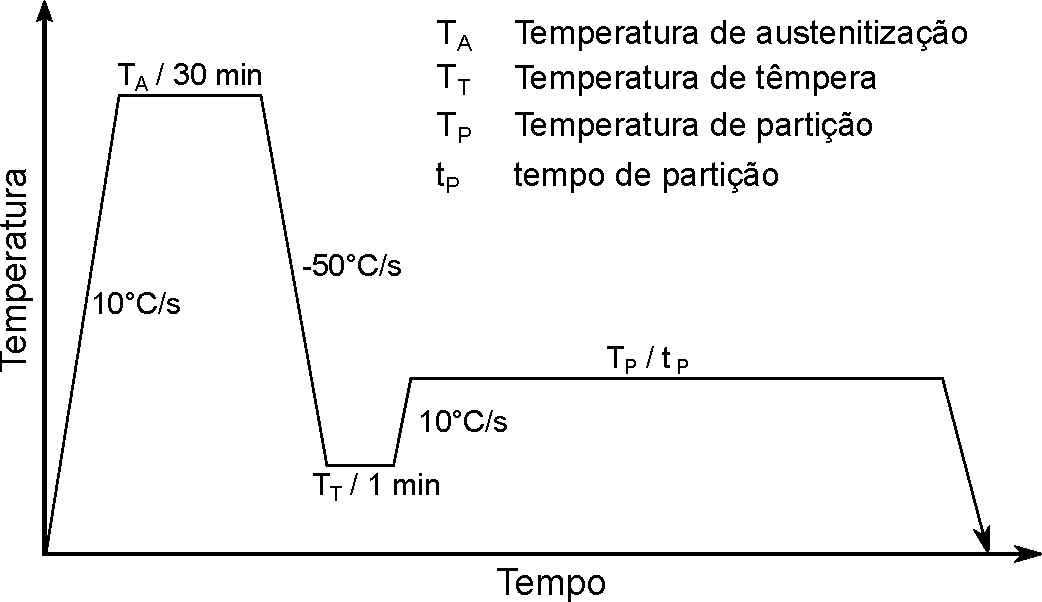
\includegraphics[width=.8\textwidth]{img/expproc_dil.pdf}
  \end{figure}
\end{frame}

\begin{frame}{Difração de raios X in situ}
  \begin{itemize}
    \item XTMS @ LNLS/LNNano: Simulador termomecânico Gleeble\textregistered{} 3S50 + DRX luz síncrotron
    % \item Aquecimento por efeito Joule (passagem de corrente pela amostra)
    \item Aquisição em tempo real de padrões de DRX $\rightarrow$ Evolução de frações de fase e seus respectivos parâmetros de rede
  \end{itemize}

  \begin{figure}
    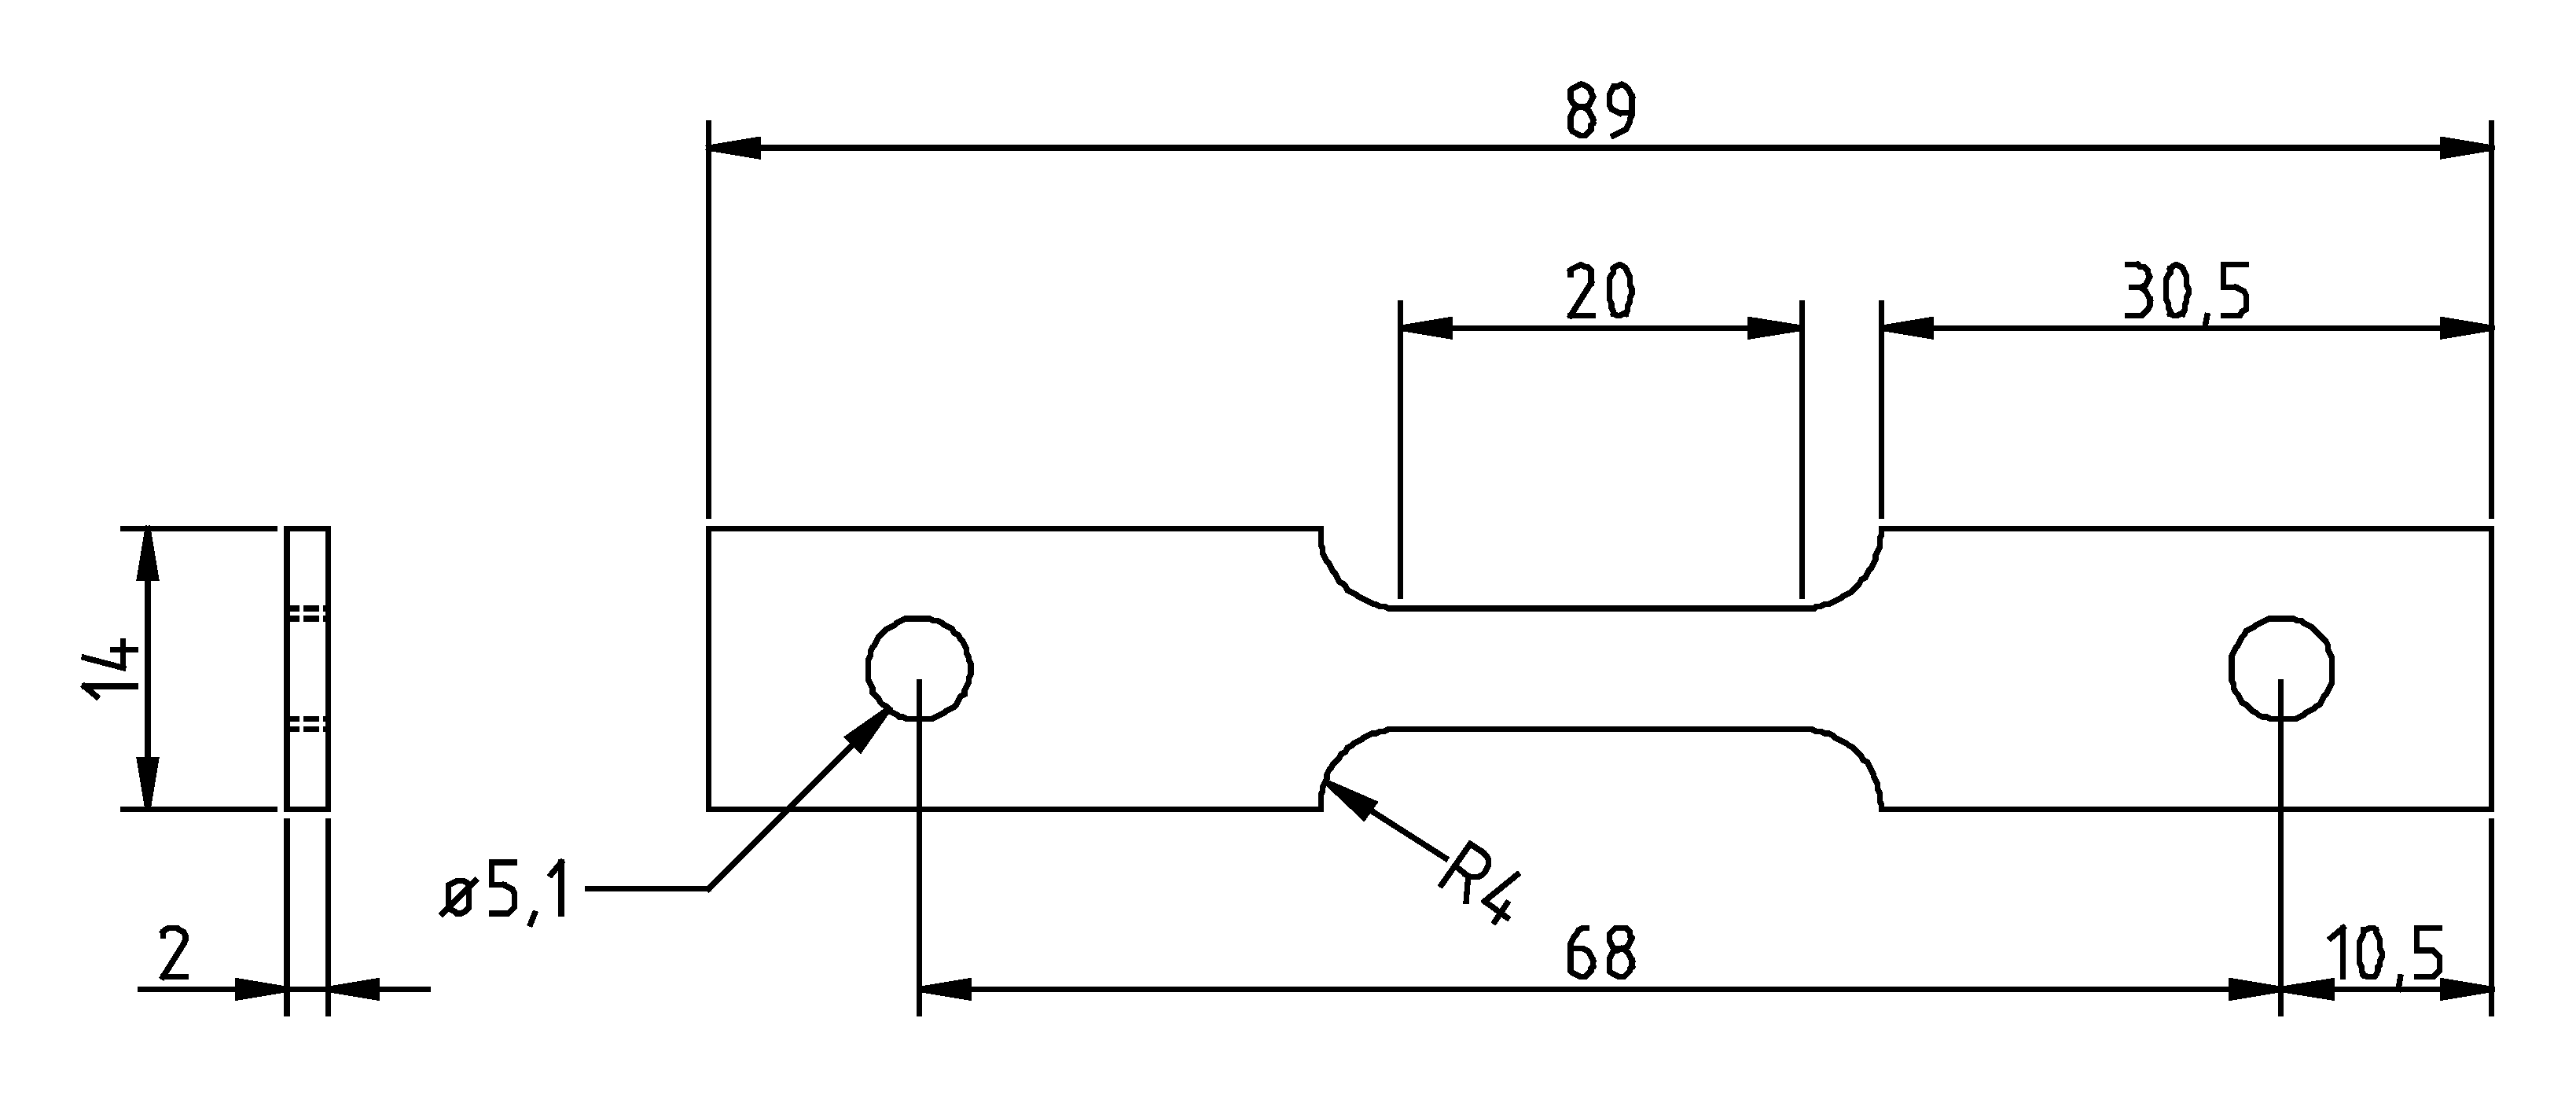
\includegraphics[width=.8\textwidth]{../tese/img/CPXTMS.pdf}
  \end{figure}
\end{frame}

\begin{frame}{Material e métodos}{DRX in situ}
  \begin{itemize}
    \item $T_T$ = \SI{170}{\degreeCelsius}
    \item $T_P$ = 300, 375, \SI{450}{\degreeCelsius} / 2~h

    \item Energia do feixe: 12~keV $\rightarrow \lambda$ = 1,033~\AA
    \item Geometria $\omega-2\theta$; $\omega$ fixo em 15°
    \item Dois detetores multicanal Mythen 1K com 1280 pixels cada
    \item Aquisições: detetores posicionados a 31° $\rightarrow$ 26°--47° (picos (111) e (200) de $\gamma$ e (110) e (200) de $\alpha$); acq. feitas a cada 3,5~s
  \end{itemize}

  \begin{figure}
    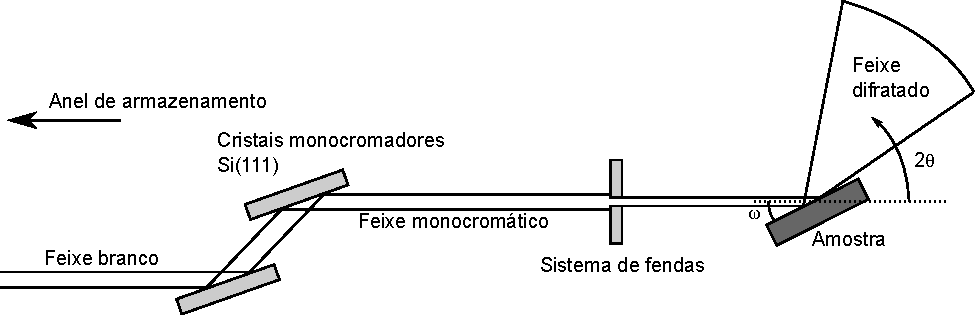
\includegraphics[width=.8\textwidth]{../tese/img/XRD1.pdf}
  \end{figure}
\end{frame}

% \begin{frame}{Material e métodos}{DRX in situ}
%   \begin{figure}
%     \centering
%     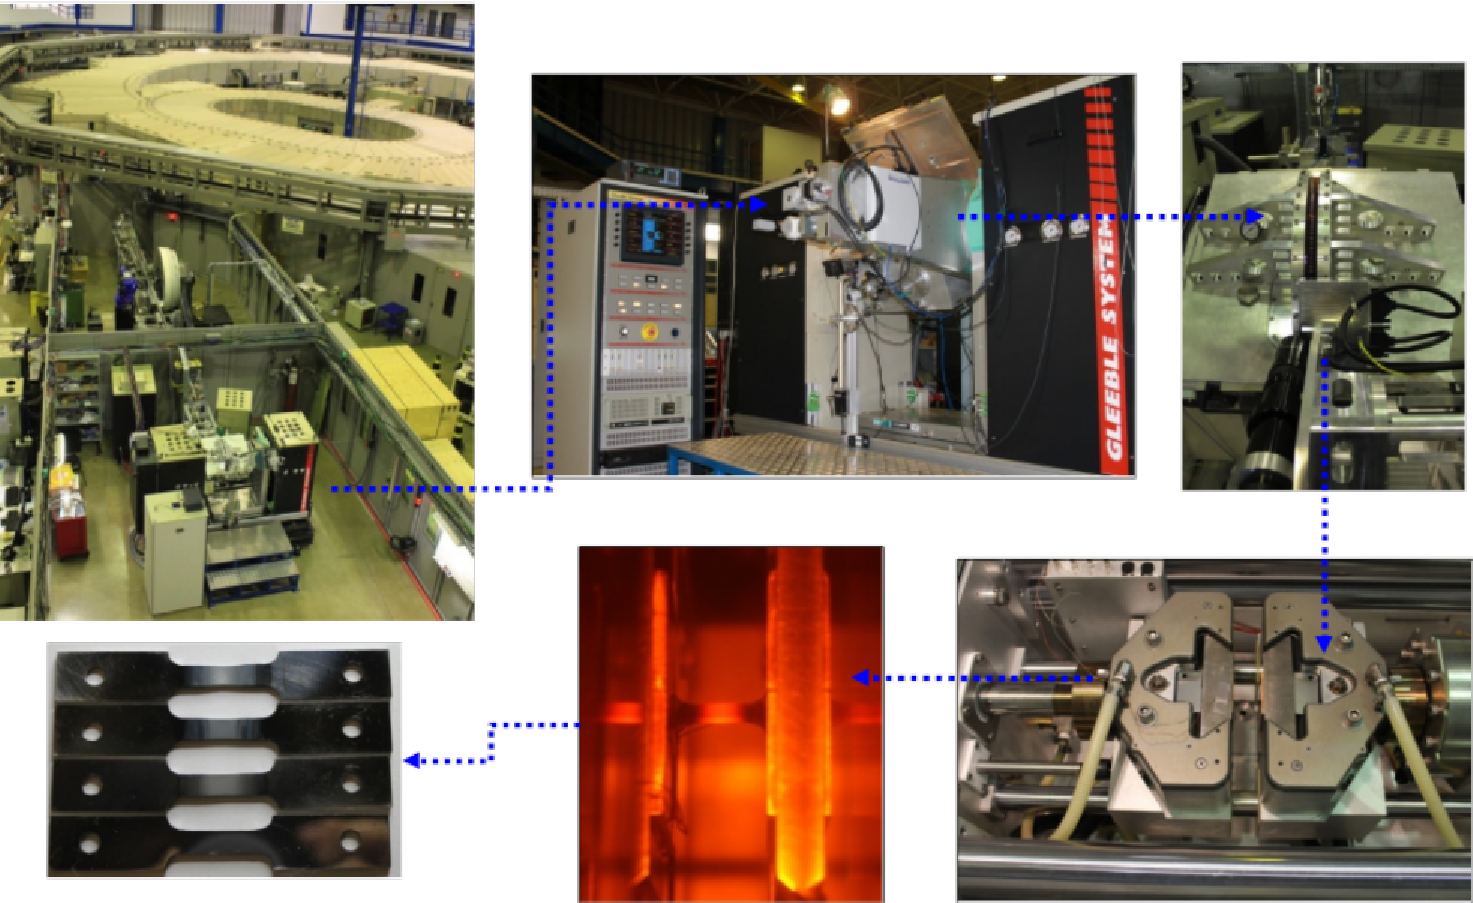
\includegraphics[width=\textwidth]{img/XTMS_facilities.pdf}
%   \end{figure}
% \end{frame}

\begin{frame}{Material e métodos}{DRX in situ}
  Tratamento de dados:
  \begin{itemize}
    \item Quantificação de fases usando procedimento convencional
    \item Determinação do parâmetro de rede da austenita ($a^\gamma$)
    \item Teor de carbono em $\gamma$ estimado pelas equações de van Bohemen\footnotemark[2] Dyson e Holmes\footnotemark[3]

    $$\frac{a^\gamma}{a_0^\gamma} = 1 + B_\gamma T + B_\gamma \Theta_D^\gamma \left[ \exp{\left( -\frac{T}{\Theta_D^\gamma} \right)}\right]$$

    $$a^\gamma = 3,5780 + 3,30\cdot10^{-2} \%w_C^\gamma + 9,5\cdot10^{-4} \%w_{Mn}^\gamma + 1,5\cdot10^{-3} \%w_{Cu}^\gamma$$
  \end{itemize}

  \footnotetext[1]{Stock S, Cullity B. Elements of X-ray diffracion. Prentice Hall, New Jersey, 2001}
  \footnotetext[2]{van Bohemen SMC. Scr Mater 2013;69:315.}
  \footnotetext[3]{Dyson DJ, Holmes B. J Iron Steel Inst 1970;208:469.}
\end{frame}

% \begin{frame}{Material e métodos}{DRX insitu}
%   \tikzset{block/.style={rectangle, draw, text width=15em, rounded corners, minimum width=3.5cm}}
%   \tikzset{title/.style={rectangle, text centered, text width=15em, minimum width=3.5cm, font=\bfseries}}
%   \tikzset{figure/.style={rectangle, text width=20em, minimum width=3.5cm}}
%   \tikzset{line/.style={draw, -latex}}


%   \scalebox{0.55}{
%     \begin{tikzpicture}
%       \node[block,text centered](raw){Dados brutos};
%       \node[block, below=1cm of raw](Gauss){Ajuste dos picos por função de Gauss\footnotemark[1]:\\
%         $I = I_0 \exp{\left[-\left(\frac{2\theta - 2\theta_0}{w}\right)^2\right]}$\alert{ + bck}};
%       \node[block, left=1cm of Gauss](integral){Integração dos picos:\\
%         $A = \int\limits_{-\infty}^{\infty} I_0 \exp{\left[-\left(\frac{2\theta - 2\theta_0}{w}\right)^2\right]} d\theta =$\\
%         $= I_0|w|\sqrt{\pi}$};
%       \node[block, below=1cm of integral](Cullity){Cálculo de $f^\gamma$ pela comparação com intensidades calculadas\footnotemark[2]:\\
%         $f^\gamma = 1 - f^\alpha = \frac{\sum A_{hkl}^\gamma/R_{hkl}^\gamma}{\sum A_{hkl}^\alpha/R_{hkl}^\alpha + \sum A_{hkl}^\gamma/R_{hkl}^\gamma}$};
%       \node[block, right=1cm of Gauss](Bragg){Lei de Bragg $\rightarrow$ converter $2\theta_0$ para $a_{TP}^\gamma$};
%       \node[block, below=1cm of Bragg](correction){Experimentos \textit{in situ} foram feitos na temp. TP $\rightarrow$ transformar $a_{TP}^\gamma$ para $a_{300K}^\gamma$ usando eq. de expansão do reticulado\footnotemark[3]:\\
%         $\frac{\Delta L^\gamma}{L_0^\gamma} = B_\gamma T + B_\gamma \Theta_D^\gamma \left[ \exp{\left( -\frac{T}{\Theta_D^\gamma} \right)}\right]$\\
%         em que $B_\gamma=24,8\times 10^{-1} K^{-1}$ e $\Theta_D^\gamma=280 K$};
%       \node[block, below=1cm of correction](Dyson){Computar teor de carbono utilizando relação entre $a^\gamma$ e $\%w_C^\gamma$ de Dyson e Holmes\footnotemark[4]:\\
%         $a^\gamma = 3,5780 + 3,30\cdot10^{-2} \%w_C^\gamma + 9,5\cdot10^{-4} \%w_{Mn}^\gamma + 1,5\cdot10^{-3} \%w_{Cu}^\gamma$};
%       \node[figure, below=0.5cm of Gauss]{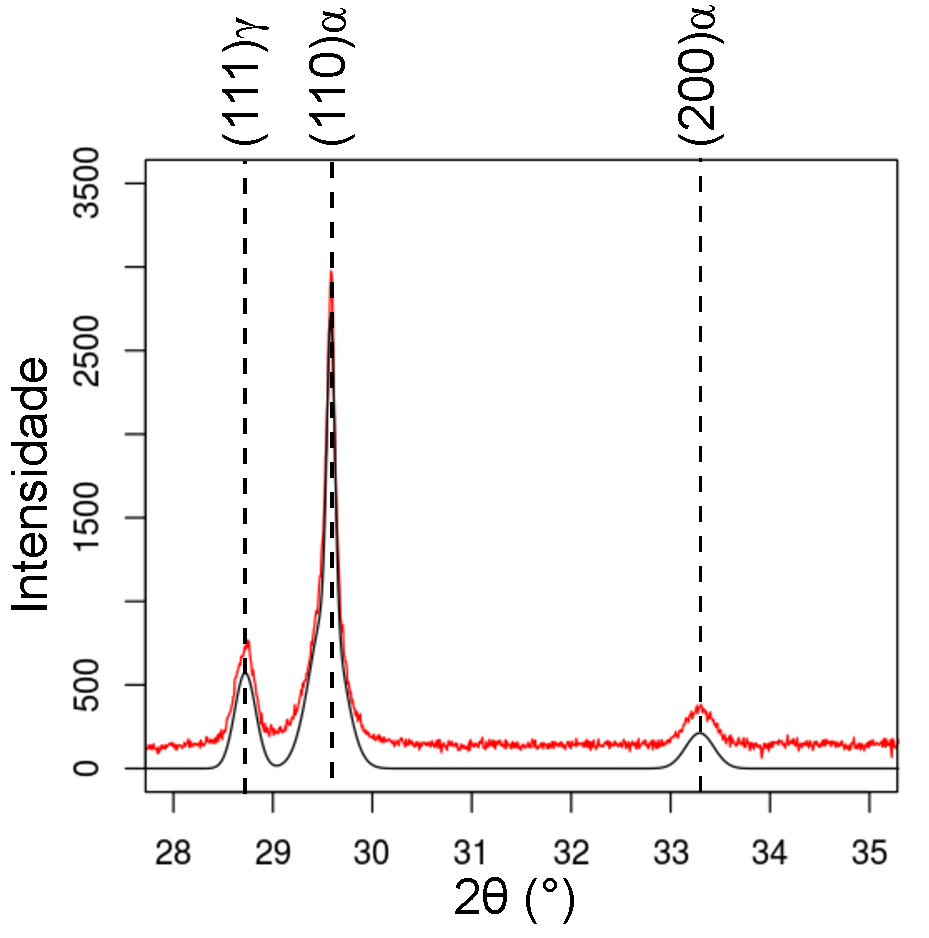
\includegraphics[width=20em]{img/peak_fitting.pdf}};
%       \node[title, above=0.5cm of integral]{Cálculo das frações volumétricas de $\alpha$ e $\gamma$};
%       \node[title, above=0.5cm of Bragg]{Cálculo do teor de carbono em $\gamma$};

%       \path[line](raw) -- (Gauss);
%       \path[line](Gauss) -- (integral);
%       \path[line](integral) -- (Cullity);
%       \path[line](Gauss) -- (Bragg);
%       \path[line](Bragg) -- (correction);
%       \path[line](correction) -- (Dyson);
%     \end{tikzpicture}
%   }
%   \footnotetext[1]{Babu SS, Specht ED, David SA, Karapetrova E, Zschack P, Peet M, Bhadeshia HKDH. Metall Mater Trans A 2005;36:3281.}
%   \footnotetext[2]{Stock S, Cullity B. Elements of X-ray diffracion. Prentice Hall, New Jersey, 2001}
%   \footnotetext[3]{van Bohemen SMC. Scr Mater 2013;69:315.}
%   \footnotetext[4]{Dyson DJ, Holmes B. J Iron Steel Inst 1970;208:469.}

% \end{frame}


\begin{frame}{Material e métodos}{Caracterização microestrutural}
  \begin{itemize}
    \item \textbf{MO}: Olympus BX60M (PMT-USP) e microscópio Nikkon (Tohoku University)
    \item \textbf{MEV}: MEV-FEG FEI Inspect F50 (PMT-USP) e JEOL JSM-7001F (Tohoku University)
    
    \begin{itemize}
      \item Preparação metalográfica convencional por lixamento e polimento até sílica coloidal
      \item MO e MEV: Ataque metalográfico com reagente Nital 2\%
    \end{itemize}

    \item \textbf{EBSD} (difração de elétrons retroespalhados): JEOL JSM-7001F com sistema TSL OIM (Tohoku University)

    \item \textbf{EPMA} (microssonda eletrônica): JEOL JXA-FE-8530 (IGc-USP)
    
    \begin{itemize}
      \item Baixo aumento: análise composicional de Mn, Si e Cu (C é estimado usando termodinâmica computacional)
      \item Alto aumento: análise composicional de C
    \end{itemize}
  \end{itemize}
\end{frame}

\begin{frame}{Material e métodos}{Difração de raios X de alta resolução}
  \begin{itemize}
    \item DRX síncrotron feita na XTMS, mas sem tratamento térmico
    \item Detetor 2D Rayonix SX165: alta resolução, alto sinal/ruído $\rightarrow$ \emph{Caracterização de carbonetos}
    \item Dados integrados azimutalmente $\rightarrow$ difratograma 1D
  \end{itemize}

  % \only<1>{
  %   \begin{figure}
  %     \begin{minipage}[c][.5\textwidth]{0.35\textwidth}%
  %     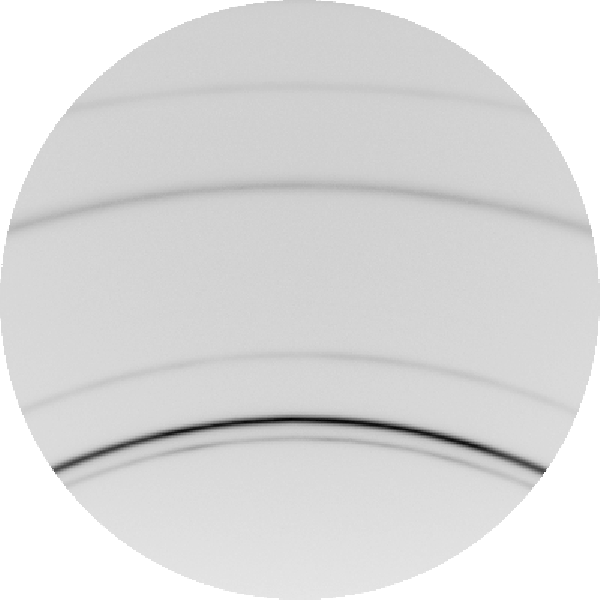
\includegraphics[width=\textwidth]{../tese/img/XTMS/PT300_detector.pdf}
  %     \end{minipage}\hfill
  %     \begin{minipage}[c][.5\textwidth]{0.6\textwidth}%
  %     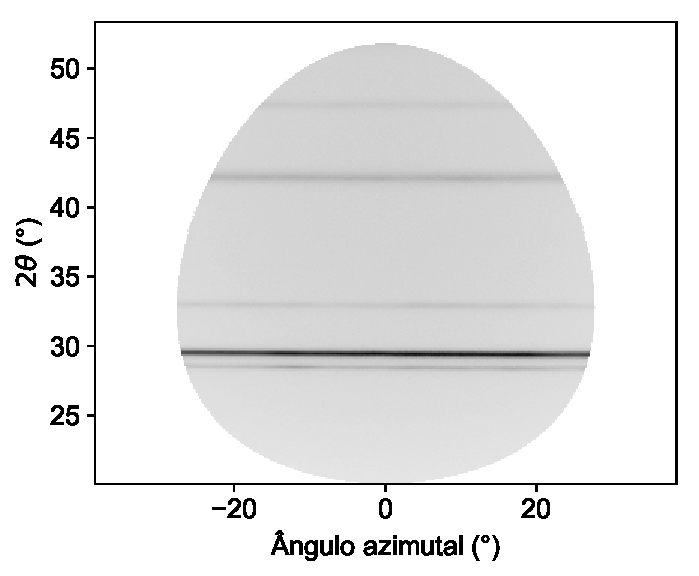
\includegraphics[width=\textwidth]{../tese/img/XTMS/PT300_spherical.pdf}
  %     \end{minipage}
  %   \end{figure}
  % }
  % \only<2>{
  %   \begin{figure}
  %     \subfloat{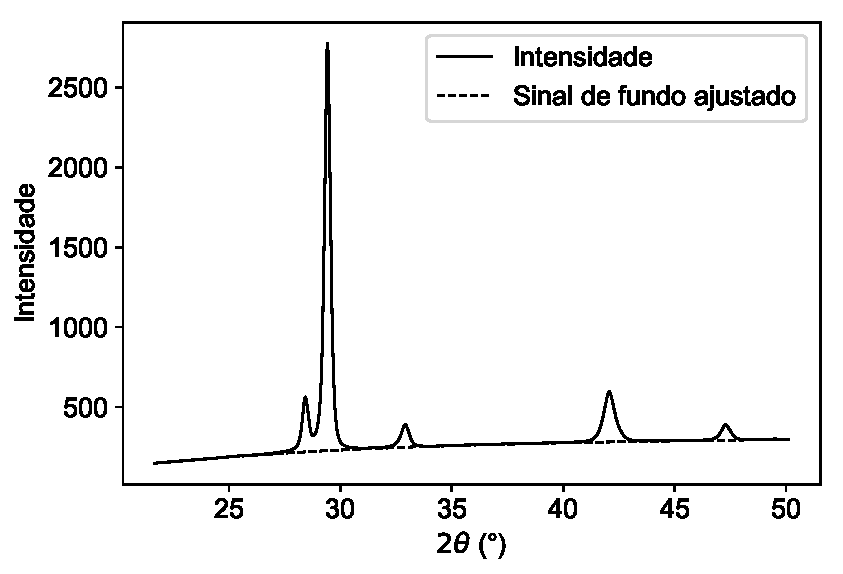
\includegraphics[width=.7\textwidth]{../tese/img/XTMS/PT300_diffractogram.pdf}}
  %   \end{figure}
  % }
\end{frame}